\chapter{Kategorisierung von Sequenzen}
Im folgenden Kapitel wird die Implementierung der Skripte vorgestellt, die unterschiedliche Eigenschaften von Sequenzen berechnen und ausgeben.
\section{Kategorisierte Eigenschaften}
Folgende Eigenschaften werden für Sequenzen ermittelt:
\begin{description}
	\item[Balance] Die Balance ist ein Maß für die \enquote{Richtung} in die eine Sequenz ausgerichtet ist. Damit wird der Tendenz zu 0 oder 1 ein Wert zugeordnet. Die Balance kann Werte zwischen 0 und 1 annehmen. Die beiden Grenzen sind ebenfalls im Wertebereich vorhanden. Eine Sequenz mit einer Balance von 0.5 gilt als ausgeglichen, das bedeutet, dass die Sequenz so viele 0er wie 1er enthält.
	\item[Frequenz] Die Frequenz ist ein Maß für die Aktivität an Wertewechseln innerhalb einer Sequenz. Ein Wert gegen 0 entspricht einer sehr inaktiven Sequenz mit nur sehr wenigen bis keinen Wertewechsel. Ein Wert von 1 steht für eine hochfrequente Sequenz, in der sehr viel Wertewechsel stattfinden.
	\item[Sub-Sequenz] Die zu analysierenden Sequenzen werden anhand ihrer Länge in kleinere Sub-Sequenzen aufgeteilt, für die ebenfalls die Balance und Frequenz berechnet werden.
\end{description}

\subsection{Berechnung Balance}

\subsubsection{Vorgehen}
Die Balance wird nach folgender Formel berechnet:
\[
Balance = \frac{Anzahl\ Wert = 1}{Gesamtl\ddot{a}nge\ der\ Sequenz}
\]
Bei einer leeren Sequenz ist der Standardrückgabewert 0.
\subsubsection{Beispiel für eine ausgeglichene Sequenz}
Die folgende Sequenz mit einer Länge von 10000 Einträgen folgt der folgenden Vorschrift und ist in Abbildung~\ref{fig:example_balance_equal} abgebildet:
\[ a_{n} =
\begin{cases}
1       & \quad \text{für } n < 5000\\
0  		& \quad \text{für } n > 5000
\end{cases}
\]

\begin{figure}[H]
	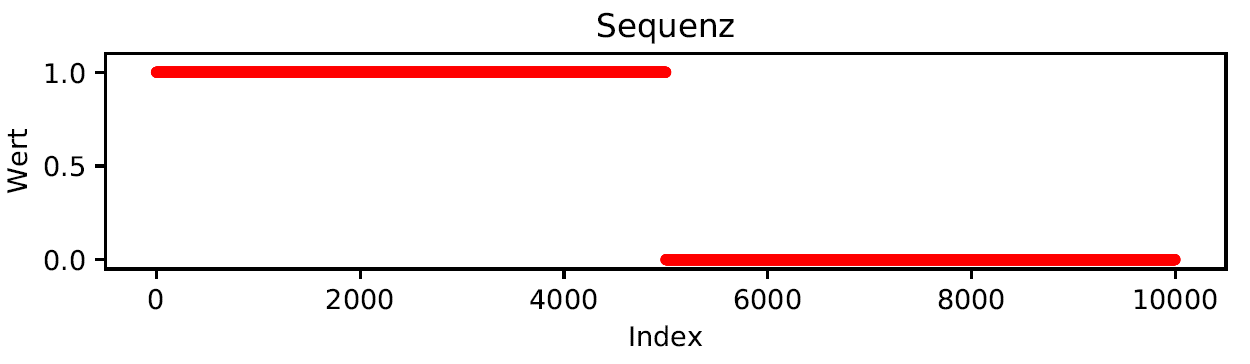
\includegraphics[width=\linewidth]{pythonImplementation/images/example_balance_equal.PNG}
	\caption[Darstellung einer ausgeglichenen Sequenz]{Stellt eine ausgeglichene (Balance = 0.5) Sequenz dar\footnotemark.}
	\label{fig:example_balance_equal}
\end{figure}
\footnotetext{Quelle: Eigene Darstellung}

Für diese Sequenz wird eine Balance von 0.5 berechnet, da es genau so viele Werte mit 1 als auch 0 gibt. 
\subsubsection{Beispiel für eine unausgeglichene Sequenz}
Die folgende Sequenz mit einer Länge von 10000 Einträgen folgt der folgenden Vorschrift und ist in Abbildung~\ref{fig:example_balance_unequal} abgebildet:
\[ a_{n} =
\begin{cases}
1       & \quad \text{für } n < 9000\\
0  		& \quad \text{für } n > 1000
\end{cases}
\]

\begin{figure}[H]
	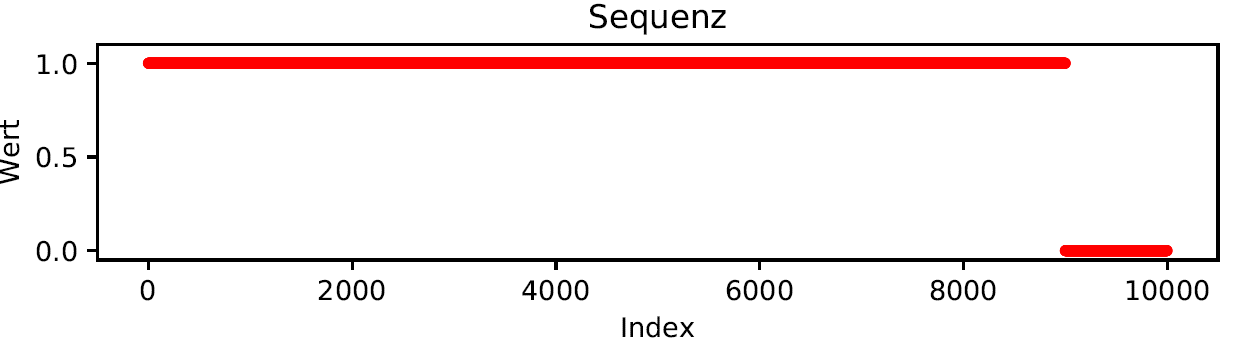
\includegraphics[width=\linewidth]{pythonImplementation/images/example_balance_unequal.PNG}
	\caption[Darstellung einer unausgeglichenen Sequenz]{Stellt eine unausgeglichene (Balance = 0.9) Sequenz dar\footnotemark.}
	\label{fig:example_balance_unequal}
\end{figure}
\footnotetext{Quelle: Eigene Darstellung}

Für diese Sequenz wird eine Balance von 0.9 berechnet, da diese deutlich Richtung 1 tendiert. 
\subsection{Berechnung der Frequenz}

\subsubsection{Vorgehen}
Die Frequenz einer Sequenz wird nach folgender Formel berechnet:
\[
Frequenz = \frac{Anzahl\ der\ Wert\ddot{a}nderungen}{Gesamtl\ddot{a}nge\ der\ Sequenz}
\]

Ein Wert <= 0.25 gilt als \enquote{Niederfrequent}, ein Wert x > 0.25 und < 0.75 gilt als \enquote{Mittelfrequent} und Werte >= 0.75 als \enquote{Hochfrequent}.
Der Standardrückgabewert einer leeren Sequenz ist 0. 

\subsubsection{Beispiel einer niederfrequenten Sequenz}
Eine niederfrequente Sequenz mit einer Länge von 10000 Einträgen ist in Abbildung~\ref{fig:example_frequence_low} abgebildet:

\begin{figure}[H]
	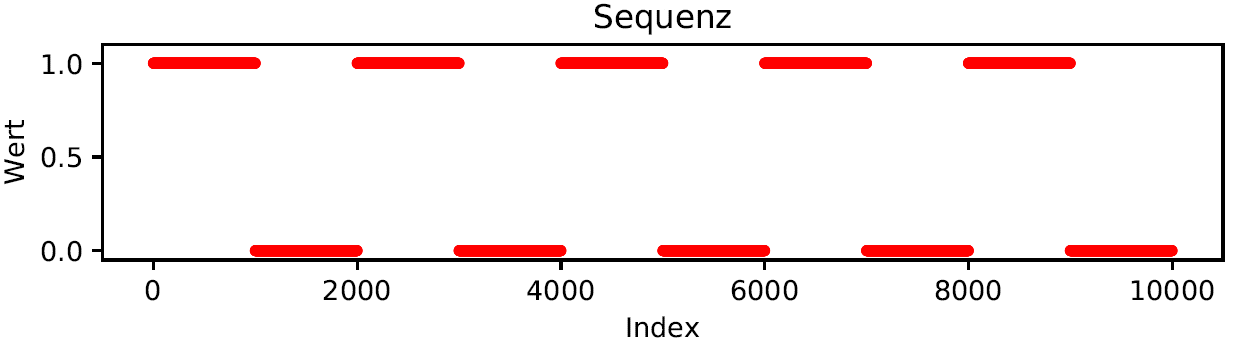
\includegraphics[width=\linewidth]{pythonImplementation/images/example_frequence_low.PNG}
	\caption[Darstellung einer niederfrequenten Sequenz]{Stellt eine niederfrequente Sequenz dar\footnotemark.}
	\label{fig:example_frequence_low}
\end{figure}
\footnotetext{Quelle: Eigene Darstellung}

Diese Sequenz hat eine berechneten Frequenzwert von 0. Die Anzahl an Wertewechsel im Verhältnis zur Länge der Sequenz ist sehr niedrig.

\subsubsection{Beispiel einer mittelfrequenten Sequenz}
Eine mittelfrequente Sequenz mit einer Länge von 10000 Einträgen ist in Abbildung~\ref{fig:example_frequence_middle} abgebildet:

\begin{figure}[H]
	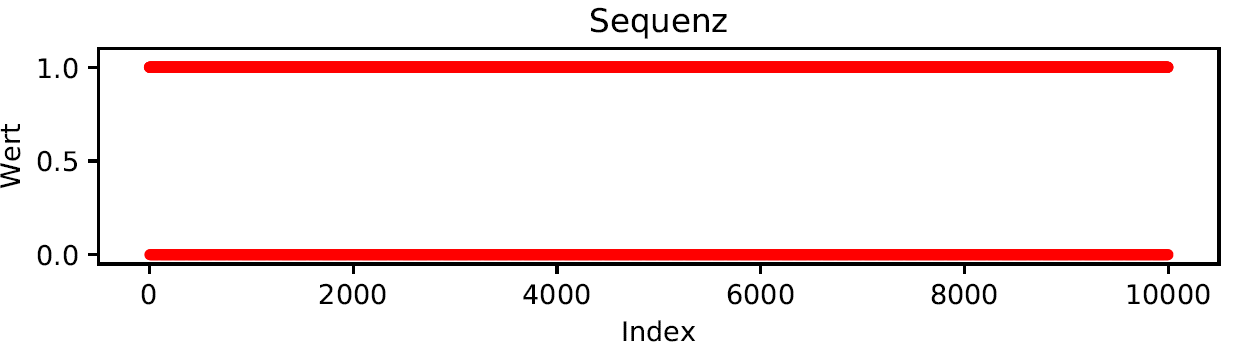
\includegraphics[width=\linewidth]{pythonImplementation/images/example_frequence_middle.PNG}
	\caption[Darstellung einer mittelfrequenten Sequenz]{Stellt eine mittelfrequente Sequenz dar\footnotemark.}
	\label{fig:example_frequence_middle}
\end{figure}
\footnotetext{Quelle: Eigene Darstellung}

Diese Sequenz hat eine berechneten Frequenzwert von 0.4 und gilt damit als mittelfrequent.

\subsubsection{Beispiel einer hochfrequenten Sequenz}
Eine hochfrequente Sequenz mit einer Länge von 10000 Einträgen ist in Abbildung~\ref{fig:example_frequence_high} abgebildet:

\begin{figure}[H]
	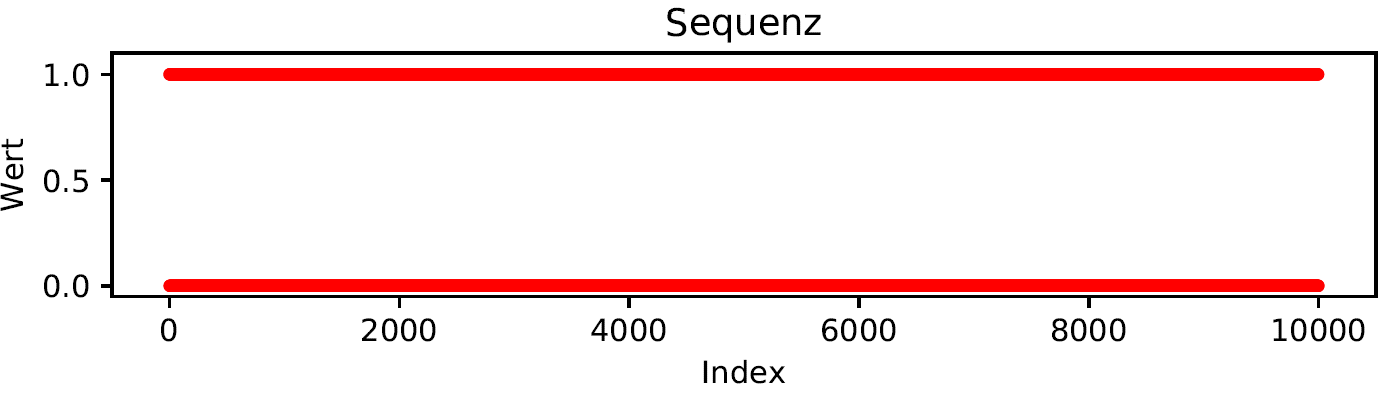
\includegraphics[width=\linewidth]{pythonImplementation/images/example_frequence_high.PNG}
	\caption[Darstellung einer hochfrequenten Sequenz]{Stellt eine hochfrequente Sequenz dar\footnotemark.}
	\label{fig:example_frequence_high}
\end{figure}
\footnotetext{Quelle: Eigene Darstellung}

Diese Sequenz hat eine berechneten Frequenzwert von 0.9 und gilt damit als hochfrequent.

\subsection{Auswertung der Sub-Sequenzen}
Im Zuge des Projekts wurde es ersichtlich, dass eine grafische Darstellung von Sequenzen in ihrer gesamte Länge nicht optimal für alle Fälle geeignet ist.
Wenn man die unterschiedlichen Sequenzen aus Abbildung~\ref{fig:example_frequence_middle} und Abbildung~\ref{fig:example_frequence_high} vergleicht, so sehen diese auf den ersten Blick identisch aus.
Bei der Auswertung der Frequenz sind diese aber unterschiedliche einzuordnen.
Dieser Effekt entsteht durch die Länge der Sequenzen und deren Darstellung in den generierten PDF Dateien.\\
Mit einer Analyse der Sequenzen in ihrer Gesamtlänge gehen auch zusätzliche Informationen verloren. Die Information ob eine Sequenz im ersten Drittel niederfrequent und zum Ende hin hochfrequent wird, kann durch einen einzelnen Zahlenwert nicht abgebildet werden.\\
Um die Unterschiede zu verdeutlichen, ist es notwendig die Sequenzen in kleinere Teilsequenzen zu unterteilen und diese zu vergleichen.

\subsubsection{Vorgehen zur Berechnung der Sub-Sequenzlängen}
Eine Sequenz wird je nach deren Länge in unterschiedlich große Teilsequenzen zerlegt. Diese Sub-Sequenzen werden ebenfalls im Bezug auf die Balance und Frequenz analysiert und die Ergebnisse werden in den entsprechenden PDF Dateien dargestellt.
Die Länge der Sub-Sequenzen wird dabei iterativ festgelegt. Das Vorgehen ist im Listing~\ref{lst:subSequenceLength} als Pseudo-Code dargestellt.\\

\lstnewenvironment{SubSequenceLength}
{\lstset{
		captionpos=b,
		frame=single,
		label={lst:subSequenceLength},
		caption={Pseudo-Code zur Festlegung der Länge der Sub-Sequenzen},
		showspaces=false,
		showtabs=false,
		breaklines=true,
		showstringspaces=false,
		breakatwhitespace=true,
		escapeinside={(*@}{@*)},
		commentstyle=\color{greencomments},
		morecomment = [l]{\#\ },
		morekeywords={ },
		keywordstyle=\color{blue},
		stringstyle=\color{black},
		morestring=[b]",
		basicstyle=\ttfamily\footnotesize,
		numberbychapter=false}}{}

\begin{SubSequenceLength}
int sequenceLength = length(sequence)
int subSequenceLength = 10

// Ensure there are at least 10 sub sequences:
while (sequenceLength / subSequenceLength ) >= 10
	SubSequenceLength is valid
	// Increase the size of the sub sequence by a factor of 10
	subSequenceLength = subSequenceLength  * 10
\end{SubSequenceLength}

Die Länge der möglichen Sub-Sequenzen startet bei 10 und wird bei jeder Iteration um den Faktor 10 erhöht. 
Die geschieht so lange, bis die Anzahl der Sub-Sequenzen 10 unterschreitet.\\
Eine Sequenz der Länge 1000 wird dabei in Sub-Sequenzen der Länge 10 und 100 aufgeteilt.
Eine Sequenz der Länge 10000 wird in Sub-Sequenzen der Länge 10, 100 und 1000 aufgeteilt.

\subsubsection{Beispiel für die analysierte Sub-Sequenzen}
Im Folgenden wird ein Beispiel für die generierten Sub-Sequenzen und deren Darstellung gegeben. 
Als Grundlage dient die in Abbildung~\ref{fig:example_subsequence} dargestellte Sequenz. 
Diese Sequenz hat eine Länge von 10000, ist mit einem Wert von 0.34 für die Frequenz mittelfrequent und gilt mit einem Balance-Wert von 0.17 als Unausgeglichen.
Man erkennt dass die Sequenz einige Intervalle mit einem Wert von 1 besitzt, wobei ein Wert von 0 klar dominiert.
Die Sequenz ist in dieser Form graphisch schwer zu analysieren, wenn man beispielsweise eine Aussage über die Länge der Ausschläge oder die Balance in Teilbereichen treffen will.

\begin{figure}[H]
	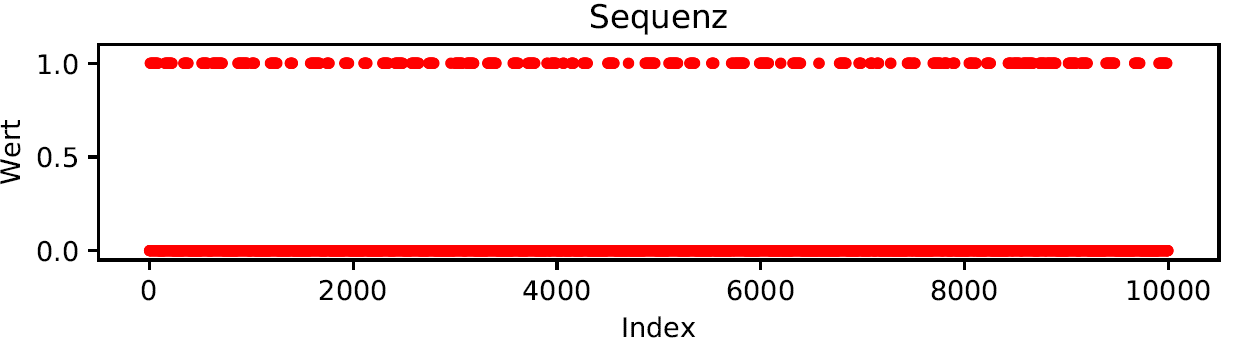
\includegraphics[width=\linewidth]{pythonImplementation/images/example_subsequences_main.PNG}
	\caption[Darstellung einer zu analysierenden Sequenz]{Stellt eine zu analysierende Sequenz dar\footnotemark.}
	\label{fig:example_subsequence}
\end{figure}
\footnotetext{Quelle: Eigene Darstellung}

Stellt man allerdings die Teilsequenzen dar, erhöht sich der Detailgrad und es wird ein Verlauf der Frequenz und der Balance ersichtlich.
Durch den erhöhten Detailgrad können die Sequenzen besser analysiert werden (falls dies notwendig ist).
\\
In Abbildung~\ref{fig:example_subsequence_balances} ist die Balance der Sub-Sequenzen dargestellt.
In dieser Darstellung ist der Verlauf der Balance erkennbar, wodurch Intervalle mit gleicher Balance besser erkennbar sind.
Die unterschiedliche Länge der Sub-Sequenzen wirkt sich dabei auf die Darstellung aus.
Je größer die Sub-Sequenz ist, desto gleichmäßiger ist die Balance.
Dadurch sind gleichmäßige Intervalle in größeren Sub-Sequenzlängen besser erkennbar als in kleinen Längen.
Kurze Ausschläge sind allerdings in kurzen Sub-Sequenzlängen besser erkennbar.

\begin{figure}[H]
	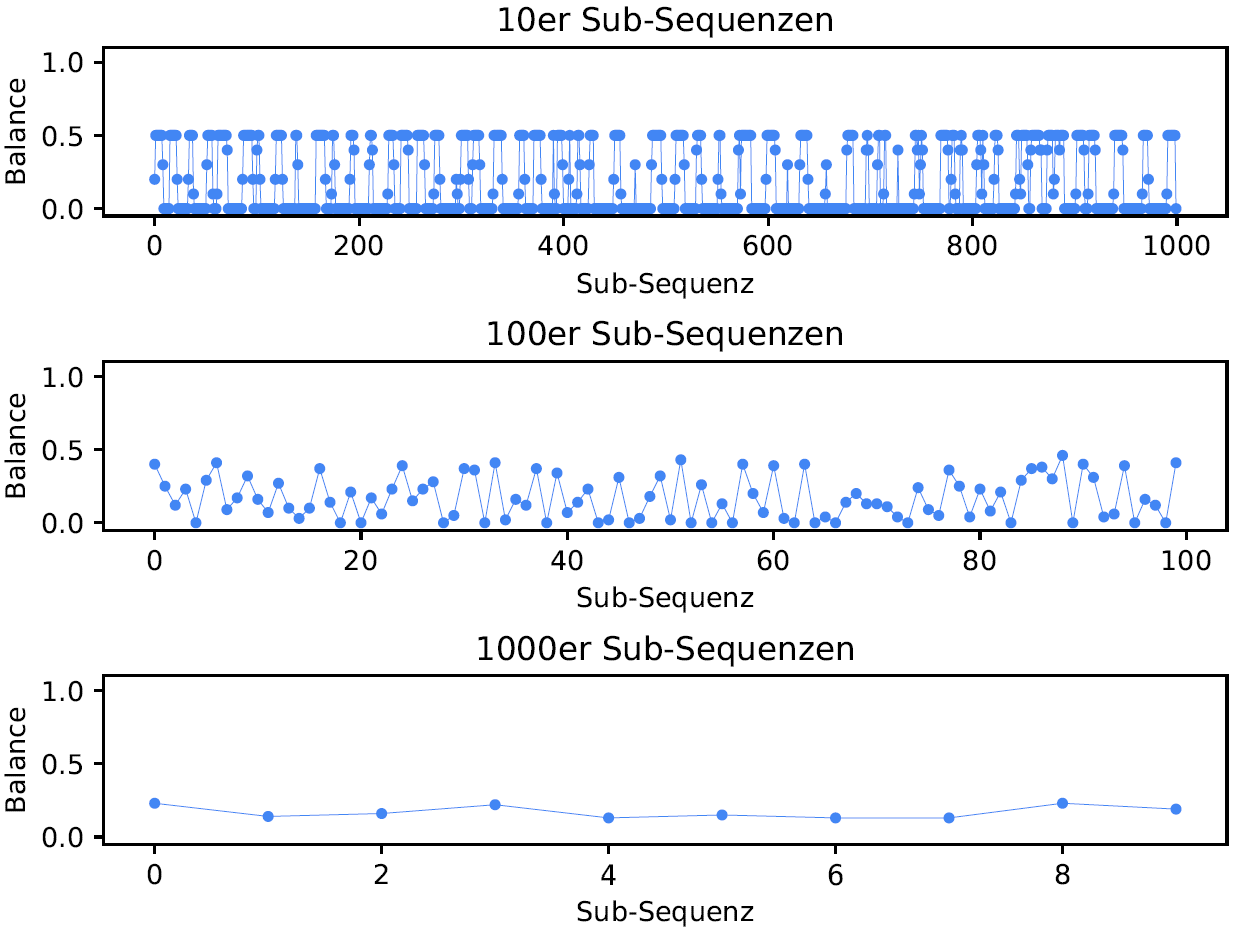
\includegraphics[width=\linewidth]{pythonImplementation/images/example_subsequences_balances.PNG}
	\caption[Darstellung der Sub-Sequenzen im Bezug auf die Balance]{Stellt die Balance der Sub-Sequenzen dar\footnotemark.}
	\label{fig:example_subsequence_balances}
\end{figure}
\footnotetext{Quelle: Eigene Darstellung}

\newpage
Analog dazu wird auch die Frequenz der Sub-Sequenzen analysiert. Das Ergebnis ist in Abbildung~\ref{fig:example_subsequence_frequences} dargestellt.

\begin{figure}[H]
	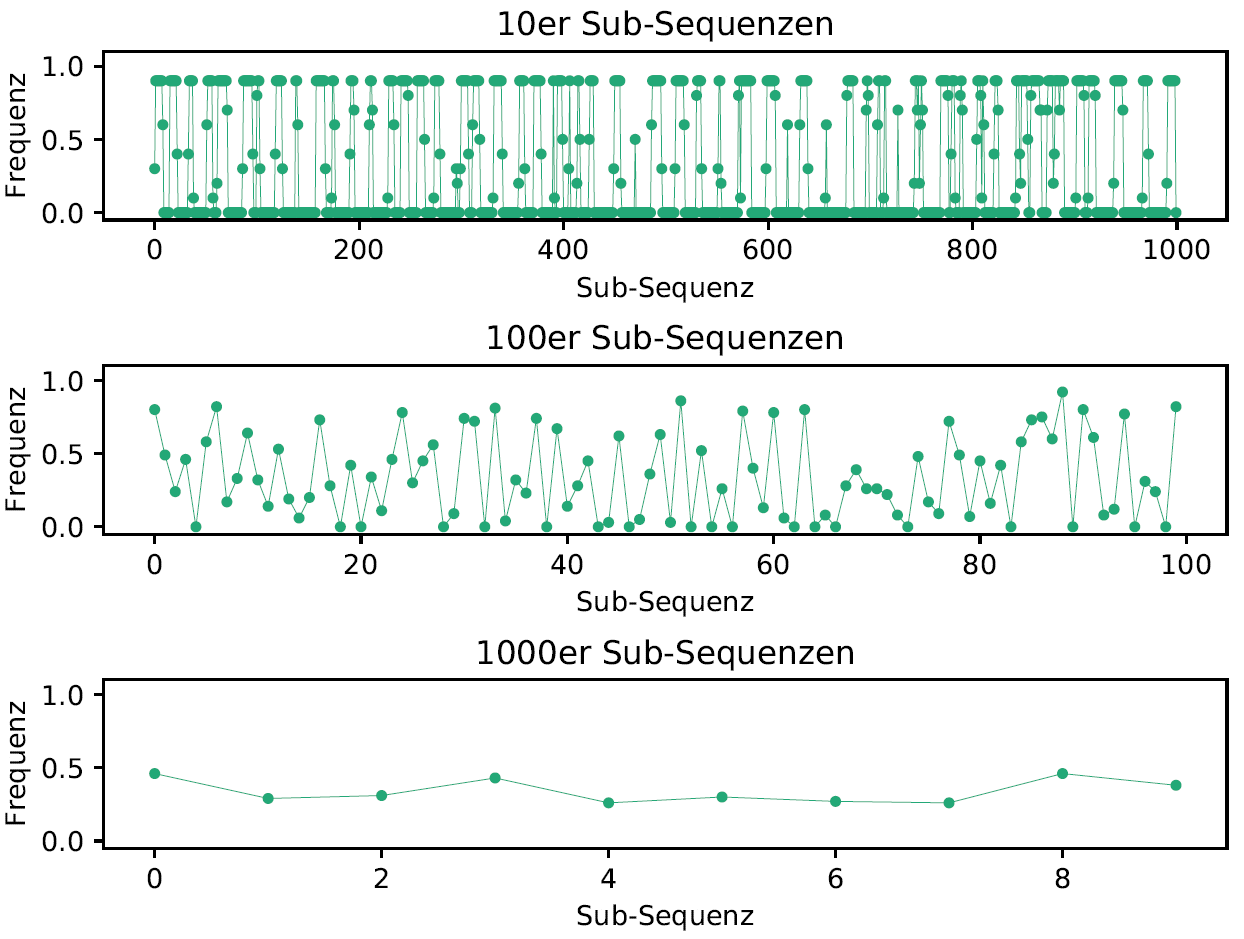
\includegraphics[width=\linewidth]{pythonImplementation/images/example_subsequences_frequences.PNG}
	\caption[Darstellung der Sub-Sequenzen im Bezug auf die Frequenz]{Stellt die Frequenz der Sub-Sequenzen dar\footnotemark.}
	\label{fig:example_subsequence_frequences}
\end{figure}
\footnotetext{Quelle: Eigene Darstellung}



\subsubsection{Vergleich über die Sub-Sequenzen}
Über die Sub-Sequenzen können die Sequenzen in manchen Fällen besser verglichen werden.
Die in Abbildung~\ref{fig:example_frequence_middle} und Abbildung~\ref{fig:example_frequence_high} dargestellten Sequenzen sehen auf den ersten Blick identisch aus.
Allerdings unterscheiden sich diese in ihrem Wert für die Frequenz (0.4 zu 0.9).
Dieser Unterschied ist auch deutlich, wenn man sich die Frequenz der entsprechenden Sub-Sequenzen anschaut.\\
Die Sub-Sequenzen der mittelfrequenten Sequenz aus Abbildung~\ref{fig:example_frequence_middle} sind in Abbildung~\ref{fig:example_frequence_middle_subsequences} dargestellt. 
Es ist nicht überraschen, dass diese sehr konstant ist und den Frequenzwert von 0.4 wiedergibt.
\begin{figure}[H]
	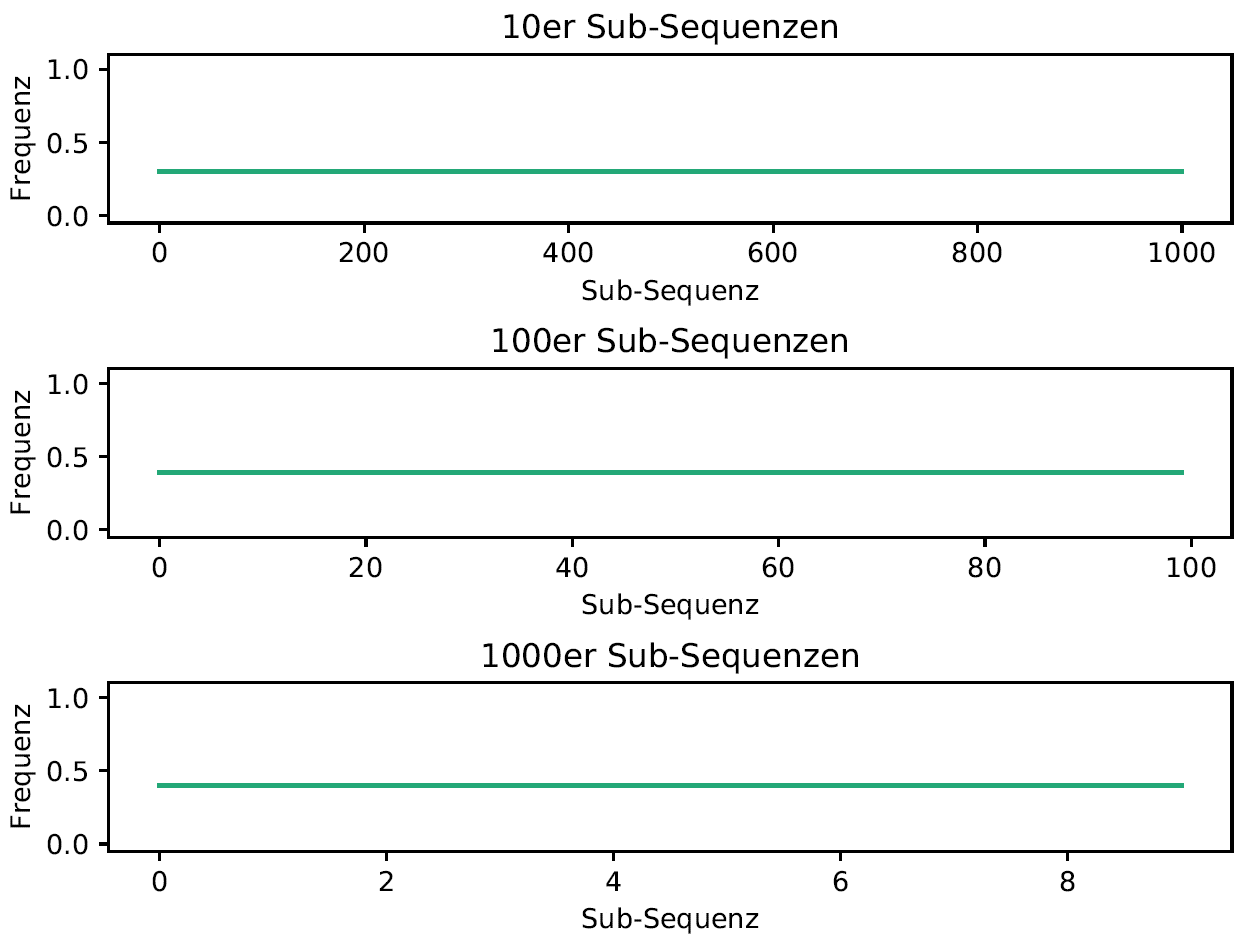
\includegraphics[width=\linewidth]{pythonImplementation/images/example_frequence_middle_subsequences.PNG}
	\caption[Darstellung der Sub-Sequenzen im Bezug auf die Frequenz einer mittelfrequenten Sequenz]{Stellt die Frequenz der Sub-Sequenzen einer mittelfrequenten Sequenz dar\footnotemark.}
	\label{fig:example_frequence_middle_subsequences}
\end{figure}
\footnotetext{Quelle: Eigene Darstellung}

Die Sub-Sequenzen der hochfrequenten Sequenz aus Abbildung~\ref{fig:example_frequence_high} zeigen hingegen ein neues Detail, welches nicht in der Gesamtansicht erkennbar ist.
Auch hier ist der hohe Wert für die Frequenz erkennbar, allerdings ist dieser nicht so gleichmäßig wie bei der mittelfrequenten Sequenz.
Es gibt einzelne Spitzen, die über die gesamte Länge der Sequenz verteilt sind. 
Die Sub-Sequenzen sind in Abbildung~\ref{fig:example_frequence_high_subsequences} dargestellt.
\begin{figure}[H]
	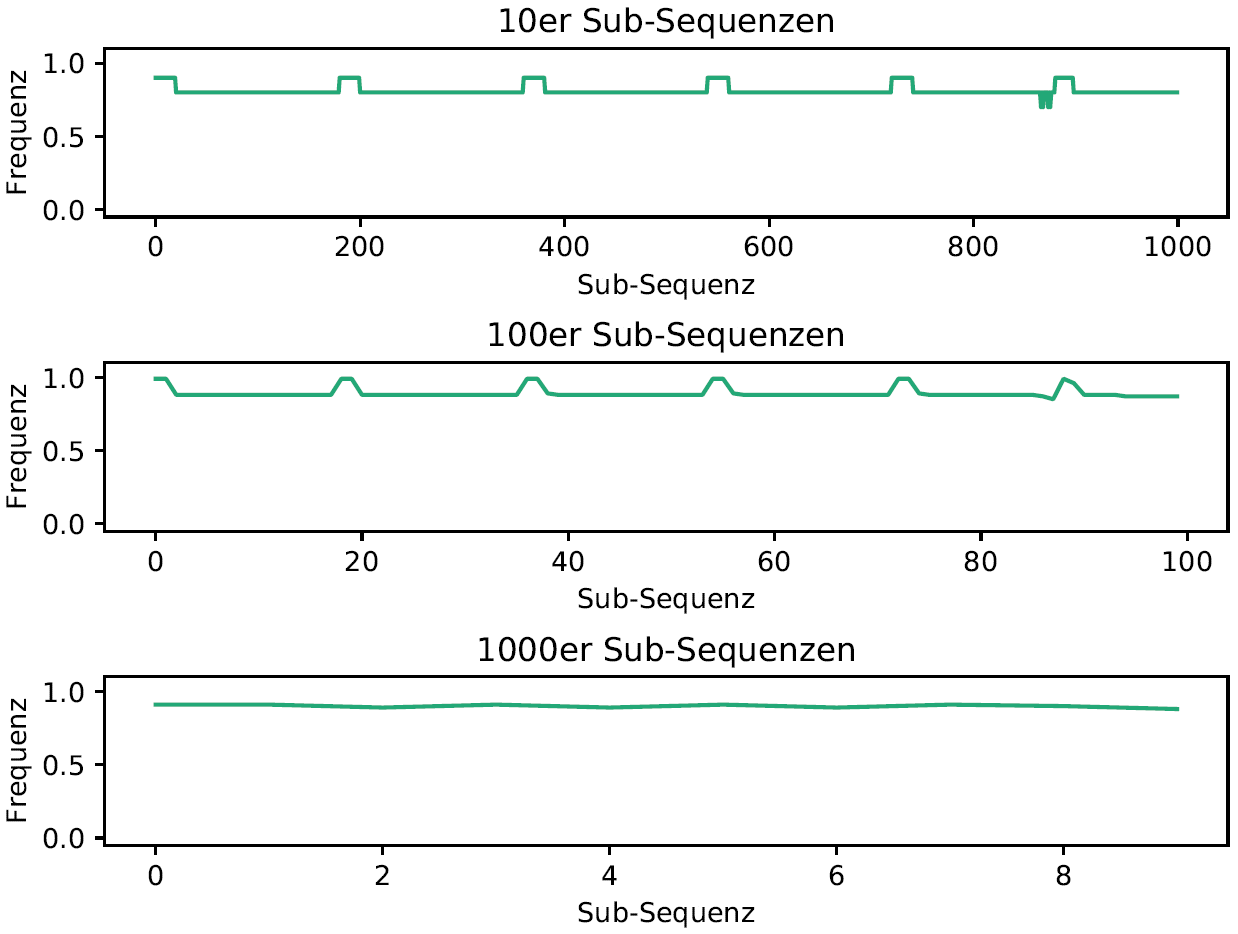
\includegraphics[width=\linewidth]{pythonImplementation/images/example_frequence_high_subsequences.PNG}
	\caption[Darstellung der Sub-Sequenzen im Bezug auf die Frequenz einer hochfrequenten Sequenz]{Stellt die Frequenz der Sub-Sequenzen einer hochfrequenten Sequenz dar\footnotemark.}
	\label{fig:example_frequence_high_subsequences}
\end{figure}
\footnotetext{Quelle: Eigene Darstellung}
